\documentclass[a4paper,14pt]{article}
\usepackage[a4paper, mag=1000, left=2.5cm, right=1cm, top=2cm, bottom=2cm, headsep=0.7cm, footskip=1cm]{geometry}
\usepackage[utf8]{inputenc}
\usepackage[T2A]{fontenc}
\usepackage[english,russian]{babel}
\usepackage{indentfirst}
%\usepackage[dvipsnames]{xcolor}
\usepackage[colorlinks]{hyperref}
\usepackage{amsmath, amsfonts, mathtools, amsthm, amssymb}
\usepackage{xparse}
\usepackage{csquotes} 
\usepackage[justification=centering]{caption}
\usepackage{cancel}
\usepackage{pdfpages}
\usepackage{graphicx}
\usepackage{float}
\newtheorem*{eg}{Пример}
\DeclareGraphicsExtensions{.png,.jpg}

\usepackage{fancyhdr}
\pagestyle{fancy}
\fancyhead[LE,RO]{\thepage}
\fancyfoot{}

\usepackage{listings}

\DeclareMathOperator{\midd}{mid}
\hypersetup{linkcolor=black}

\title{non-linear equations}
\author{Иван Золин}
\date{2023}
\thispagestyle{empty}
\begin{document}
	
	\begin{titlepage}
		\begin{center}
			\textsc{
				Санкт-Петербургский политехнический университет имени Петра Великого \\[5mm]
				Институт прикладной математики и механики\\[2mm]
				Высшая школа прикладной математики и физики            
			}   
			\vfill
			\textbf{\large
				Математическая статистика\\
				Отчёт по лабораторным работам №10 \\[3mm]
			}                
		\end{center}
		
		\vfill
		\hfill
		\begin{minipage}{0.5\textwidth}
			Выполнил: \\[2mm]   
			Студент: Золин Иван \\
			Группа: 5030102/00201\\
		\end{minipage}
		
		\hfill
		\begin{minipage}{0.5\textwidth}
			Принял: \\[2mm]
			к. ф.-м. н., доцент \\   
			Баженов Александр Николаевич
		\end{minipage}
		
		\vfill
		\begin{center}
			Санкт-Петербург \\2023 г.
		\end{center}
	\end{titlepage}
	
	\tableofcontents
	\newpage
	\listoffigures
	\newpage
	
	\section{Постановка задачи}
	Дадим общую формулировку задачи восстановления функциональной зависимости. Пусть некоторая величина $y$ является функцией от независимых переменных $x_1, x_2, ..., x_m$:
	$$y = f(\beta, x)\eqno (1)$$
	где $x = (x_1, x_2, ..., x_m)$ является вектором независимых переменных, $\beta =(\beta_1, \beta_2, ..., \beta_p)$ — вектор параметров функции. Заметим, что переменные $x_1, x_2, ..., x_m$ также называются входными, а переменные $y_1$ —
	выходной.
	
	Задача восстановления функциональной зависимости заключается в том, чтобы, располагая набором значений $x$ и $y$, найти такие $\beta_1, \beta_2, ..., \beta_p$ в выражении (1), которые соответствуют конкретной
	функции $f$ из параметрического семейства.
	
	Если функция $f$ является линейной, то можно записать
	$$y = \beta_0 + \beta_1 x_1 + ... + \beta_m x_m\eqno (2)$$
	
	В общем случае результаты измерений величин $x_1, x_2, ..., x_m$ и $y$
	являются интервальнозначными
	$$x_1^{(k)}, x_2^{(k)}, ..., x_m^{(k)}\:и\:y^{k}.$$
	Индекс $k$ пробегает значения от 1 до $n$, равного полному числу измерений.
	\newline
	\newline
	\textbf{Определение 2.2.1} Брусом неопределенности $k$-го измерения функциональной зависимости будем называть интервальный вектор-брус, образованный интервальными результатами измерений с одинаковыми значениями индекса $k$ [1]:
	$$(x_{k1}, x_{k2}, ..., x_{km}, y_k)\subset\mathbb{R}^{m+1}, k=1, 2, ..., n. \eqno (3) $$
	Брус неопределенности измерения является прямым декартовым
	произведением интервалов неопределенности независимых переменных
	и зависимой переменной.
	\newpage
	\section{Теория}
	\textbf{Данные выборки.} Имеется выборка данных $\textbf{X}_1$ с интервальной
	неопределённостью. Число отсчётов в выборке равно 200.
	
	\begin{figure}[H]
		\begin{center}
			\begin{tabular}{ccc}
				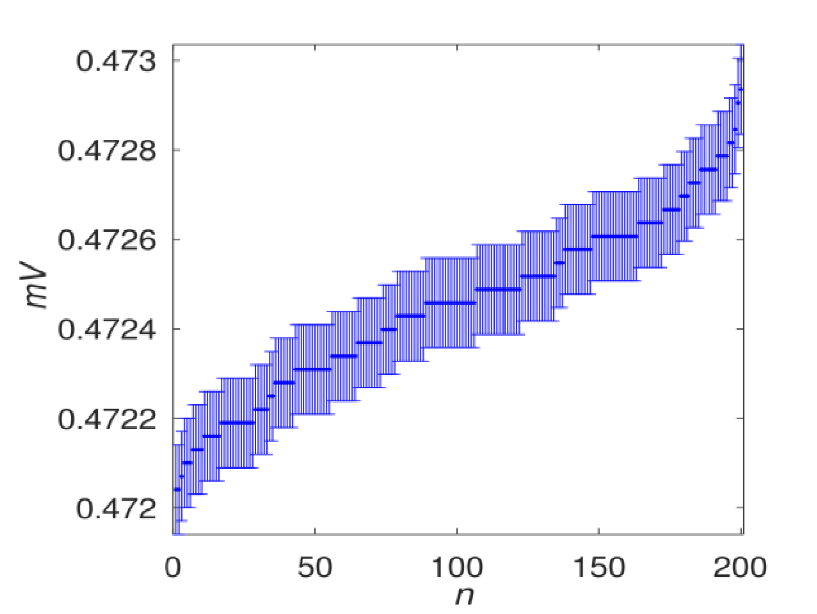
\includegraphics[scale=0.8]{../image/problem1.png}
			\end{tabular}
		\end{center}
		\caption{Диаграмма рассеяния выборки $X_1$ с уравновешенным интервалом погрешности} 
	\end{figure}
	
	На Рис. 1 представлены данные с прибора [23] с учётом погрешности измерительного прибора.
	
	Построим линейную модель данных и посмотрим, насколько удачно
	она описывает линейный тренд.
	
	\textbf{Варьирование неопределённости измерений.} Если величину коррекции каждого интервального наблюдения выборки выражать коэффициентом его уширения $\omega_i\geq1$, а общее изменение выборки характеризовать суммой этих коэффициентов, то минимальная коррекция выборки в виде вектора коэффициентов $\omega = (\omega_1, ..., \omega_n)$, необходимая для совместности задачи построения зависимости $x = \beta_0 + \beta_1 * i$ может быть найдена решением задачи условной оптимизации
	$$найти \min\limits_{\omega, \beta} \sum\limits_{i=1}^{n} \omega_i \eqno (4)$$
	при ограничениях
	\[
	\begin{cases}
		mid\:x_i-\omega_i\epsilon_i\leq\beta_0 + \beta_1 * i\leq mid\:x_i+\omega_i\epsilon_i,\\
		\omega_i\geq1,
	\end{cases}
	i = 1, ..., n.\eqno (5)\]
	
	Результирующие значения коэффициентов $\omega_i$, строго превосходящие единицу, указывают на наблюдения, которые требуют уширения интервалов неопределённости для обеспечения совместности данных и модели.
	
	Проведём вычисление параметров линейной регрессии по данным
	интервальной выборки $\textbf{X}_1$ с использованием программ С.И.Жилина [8] и оформленных применительно к задаче на [23]. Синтаксис вызова программы
	$$[tau, w, yint] = DataLinearModel(input1, epsilon0) \eqno (6)$$
	В (6) входами программы служат значения $mid\:\textbf{X}_1$ и величин
	неопределённости $\epsilon$, а выходами tau — значения параметров регресии
	$\beta_0, \beta_1\:и\:w$ — вектор весов расширения интервалов.
	
	На Рис. 2 красным цветом приведена регрессионная прямая.
	
	Вычисления с использованием программы (6) дают следующие
	результаты для регрессионных коэффициентов
	$$\beta_0 = tau(1) = 4.7203e - 01,\eqno (7)$$
	$$\beta_1 = tau(2) =  4.0915e - 06.\eqno (8)$$
	Все компоненты вектора $\omega$ оказались равны 1, то есть, расширения интервалов измерений не понадобилось. Таким образом, величина (4)
	равна числу элементов выборки.
	$$\min\limits_{\omega, \beta} \sum\limits_{i=1}^{n} \omega_i = 200\eqno (9)$$
	
	Недостатком полученного решения с единичными значениями $\omega_i$
	является неучёт расстояний точек регрессионной зависимости до данных интервальной выборки. Таким образом, прямая с параметрами
	
	\begin{figure}[H]
		\begin{center}
			\begin{tabular}{ccc}
				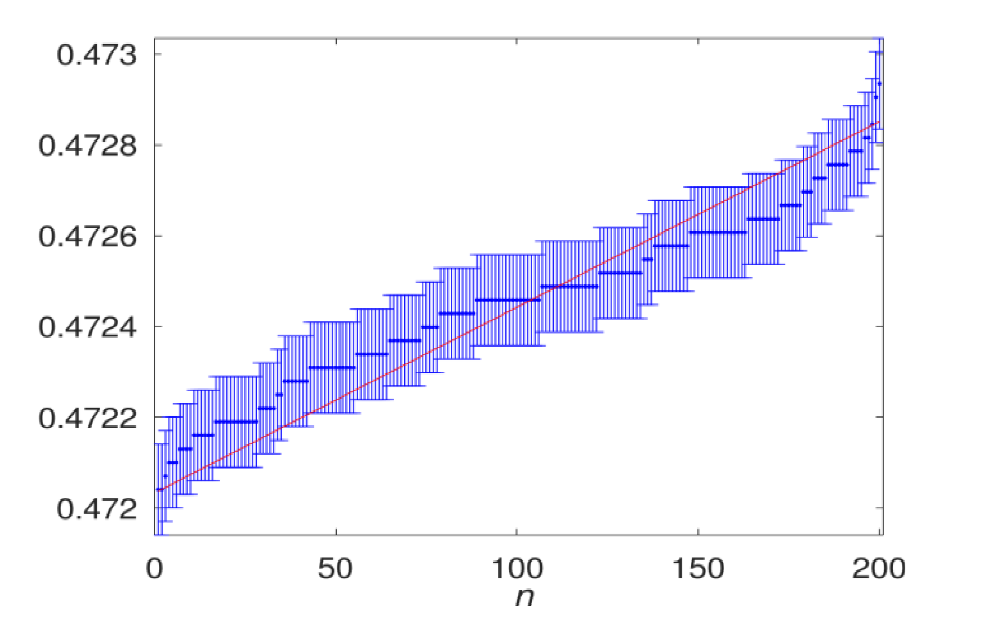
\includegraphics[scale=0.8]{../image/problem2.png}
			\end{tabular}
		\end{center}
		\caption{Диаграмма рассеяния выборки $X_1$ и регрессионная прямая по модели (4) и (5)} 
	\end{figure}
	
	(7) и (8) «не чувствует» отклонений измерений от прямой на концах выборки — неопределённости измерений достаточно велики, чтобы
	покрыть этот эффект.
	
	\textbf{Варьирование неопределённости измерений с расширением и
		сужением интервалов.} Выясним, что даёт решение задачи оптимизации другим способом, с расширением и сужением интервалов.
	
	Поставим задачу условной оптимизации следующим образом:
	$$найти \min\limits_{\omega, \beta} \sum\limits_{i=1}^{n} \omega_i \eqno (10)$$
	при ограничениях
	\[
	\begin{cases}
		mid\:x_i-\omega_i\epsilon_i\leq\beta_0 + \beta_1 * i\leq mid\:x_i+\omega_i\epsilon_i,\\
		\omega_i\geq0,
	\end{cases}
	i = 1, ..., n.\eqno (11)\]
	
	Отличие постановки от (4) и (5) состоит в том, что интервалы
	измерений могут как расширяться в случае $\omega_i\geq1$, так и сужаться при
	$0\leq\omega_i\leq1$.
	Вычисление параметров линейной регрессии по данным интервальной выборки $\textbf{X}_1$ производится как и в случае (6) с использованием программ С.И.Жилина [8] и оформленных применительно к задаче на [23]. Синтаксис вызова программы
	$$[tau, w, yint] = DataLinearModelZ(input1, epsilon0)\eqno (12)$$
	Входы и выходы функции DataLinearModelZ такие же, как и для
	DataLinearModelZ (6). 
	
	На Рис. 3 красным цветом приведена регрессионная прямая.
	
	\begin{figure}[H]
		\begin{center}
			\begin{tabular}{ccc}
				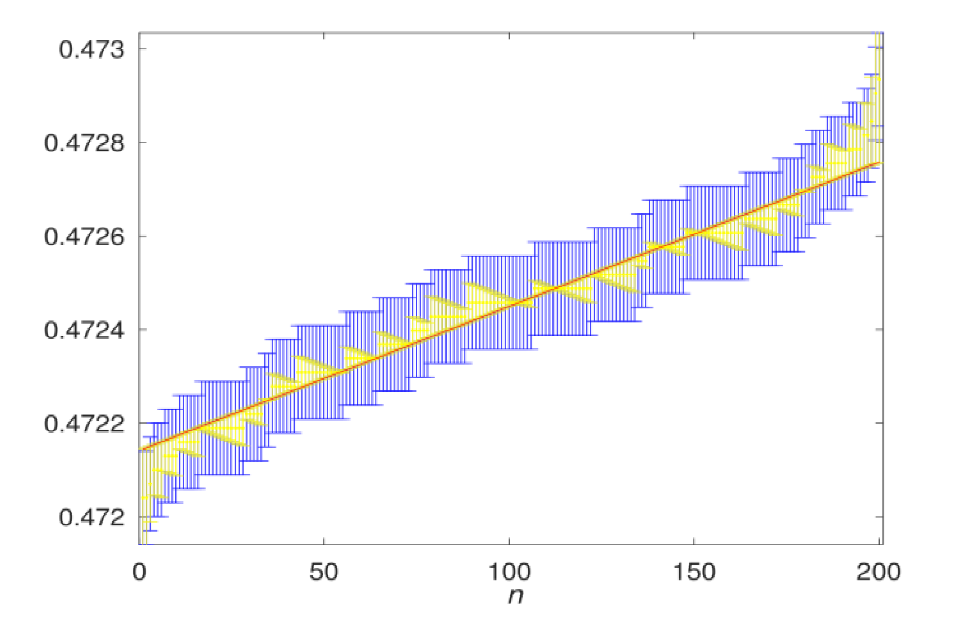
\includegraphics[scale=0.8]{../image/problem3.png}
			\end{tabular}
		\end{center}
		\caption{Диаграмма рассеяния выборки $X_1$ и регрессионная прямая по модели (10) и (11)} 
	\end{figure}

	Жёлтым цветом на Рис. 3 показаны скорректированные интервалы выборки $\textbf{X}_1$. Небольшая часть интервалов на границах области расширилась, а большинство интервалов в диапазоне замеров примерно от 20 до 180 — сузилось.
	
	Величина меры (4) уменьшилась более, чем в 4 раза.
	$$\min\limits_{\omega, \beta} \sum\limits_{i=1}^{n} \omega_i = 45.7\leq200\eqno (13)$$
	
	Таким образом, постановка задачи с возможностью одновременного
	увеличения и уменьшения радиусов неопределённости измерений позволяет более гибко подходить к задаче оптимизации.
	
	На Рис. 4 приведены графики векторов $\omega_0$ и $\omega_1$, полученных при
	использовании двух рассмотренных подходов.
	
	В конкретном случае график вектора $\omega_0$ для постановки задачи оптимизации (10) и (11) содержит большое количество информации.
	
	Например, задавшись каким-то порогом $\alpha$: $0<\alpha\leq1$, можно выделить области входного аргумента $\Psi$, в которых регрессионная зависимость хуже соотвествует исходным данным. Например:
	$$\Psi = \arg_i \omega_i \geq\alpha \eqno (14)$$
	Для конкретного примера имеем две области $\Psi$ в начале и конце области данных.
	
	\begin{figure}[H]
		\begin{center}
			\begin{tabular}{ccc}
				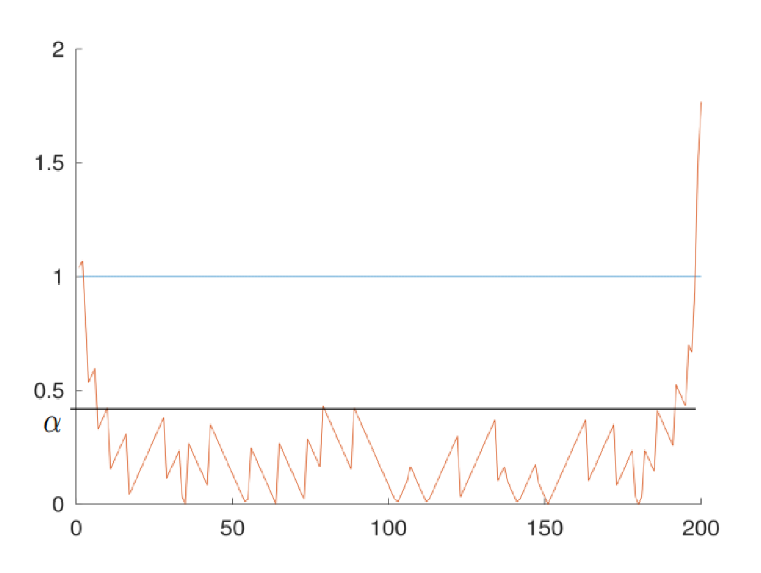
\includegraphics[scale=0.8]{../image/problem4.png}
			\end{tabular}
		\end{center}
		\caption{Векторы $\omega_1$ и $\omega_0$} 
	\end{figure}

	Для объективного использования этого приёма параметр $\alpha$ можно
	брать, например, из анализа гистограммы распределения вектора вектора $\omega$.
	
	Использование выделения «подозрительных» областей даёт основу для других приёмов. Например, для построения кусочно-линейной регрессионной зависимости.
	
	\textbf{Анализ регрессионных остатков.} В теоретико-вероятностной математической статистике анализ регрессионных остатков — один из приёмов оценки качества регрессии.
	
	Приведём пример пояснения этого приёма. «Если выбранная регрессионная модель хорошо описывает истинную зависимость, то остатки должны быть независимыми, нормально распределенными случайными величинами с нулевым средним, и в
	их значениях должен отсутствовать тренд. Анализ регрессионных остатков — это процесс проверки выполнения этих условий.»
	https://wiki.loginom.ru/articles/discrepancy.html
	
	В случае интервальных выборок мы не задаёмся вопросом о виде
	распределения остатков, а будем использовать те возможности которые
	появляются при описании объектов и результатов вычислений в виде
	интервалов.
	
	На Рис. 5 приведена диаграмма рассеяния регрессионных остатков выборки $\textbf{X}_1$ по модели (4) и (5).
	
	\begin{figure}[H]
		\begin{center}
			\begin{tabular}{ccc}
				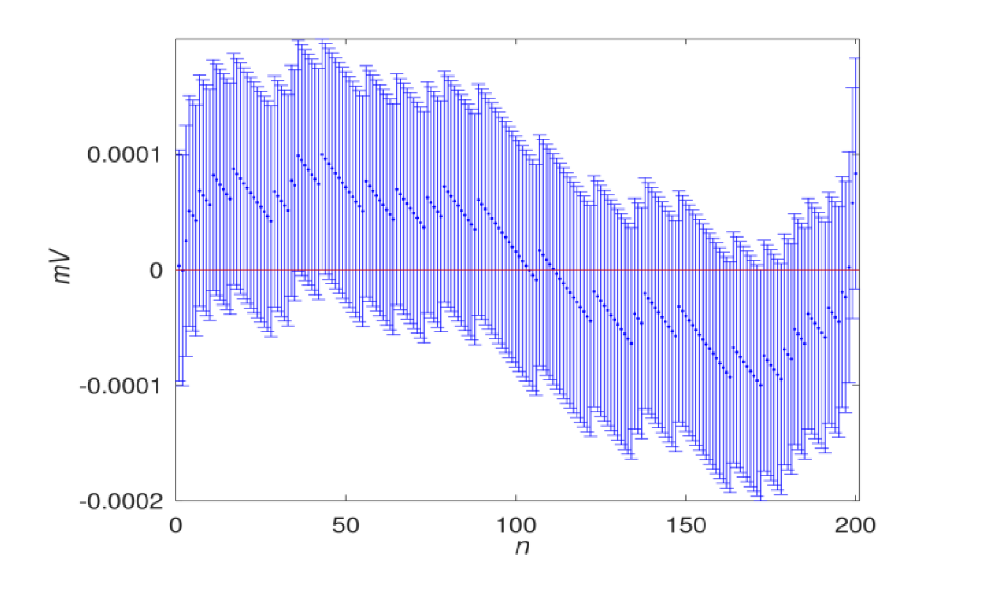
\includegraphics[scale=0.8]{../image/problem5.png}
			\end{tabular}
		\end{center}
		\caption{Диаграмма рассеяния по модели (4) и (5)} 
	\end{figure}

	На Рис. 6 приведена диаграмма рассеяния регрессионных остатков выборки $\textbf{X}_1$ по модели (10) и (11).
	
	\begin{figure}[H]
		\begin{center}
			\begin{tabular}{ccc}
				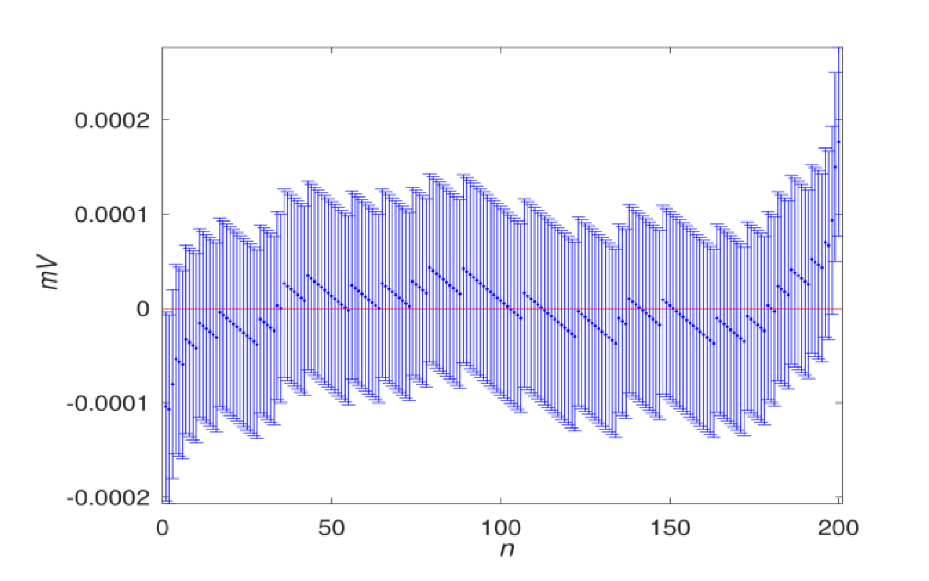
\includegraphics[scale=0.8]{../image/problem6.png}
			\end{tabular}
		\end{center}
		\caption{Диаграмма рассеяния по модели (10) и (11)} 
	\end{figure}

	Из сравнения Рис. 5 и На Рис. 6 видно, что интервальные выборки остатков получились с весьма разными свойствами. Формально диаграмма рассеяния на первом рисунке `уже, то есть внешняя оценка более компактная. В то же время вторая диаграмма рассеяния выглядит более естественно.
	
	На Рис. 7 приведены графики частот элементарных подинтервалов при вычислении интервальной моды для двух моделей.
	
	\begin{figure}[H]
		\begin{center}
			\begin{tabular}{ccc}
				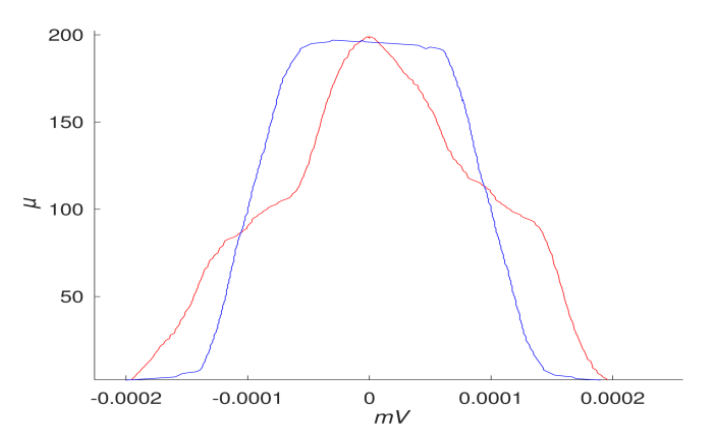
\includegraphics[scale=0.8]{../image/problem7.png}
			\end{tabular}
		\end{center}
		\caption{Частоты элементарных подинтервалов регрессионных остатков выборки $X_1$ по модели (4) и (5) — красный график, и (10) и (11) — синий график} 
	\end{figure}

	Как и в случае анализа диаграмм рассеяния, второй график выглядит более естественно. Его внутренняя оценка существенно шире, что соотвествует большей устойчивостью к возмущениям данных.
	
	К остаткам можно применить и другие меры совместности оценки
	постоянной величины, описанные ранее.
	$$mode\:\textbf{X}^1 = ...\eqno (15)$$
	$$Ji(\textbf{X})^1 = ...\eqno (16)$$
	$$\vdots\eqno (17)$$
	$$mode\:\textbf{X}^2 = ...\eqno (18)$$
	$$Ji(\textbf{X})^2 = ...\eqno (19)$$
	$$\vdots\eqno (20)$$
	здесь $\textbf{X}^{1,2}$ — регрессионные остатки выборки $\textbf{X}_1$, вычисленные с использованием разных условий оптимизации.
	
	\textbf{Информационное множество задачи.} Интервальные оценки параметров.
	
	Один из главных вопросов при построении регрессии – оценивание
	её параметров. В зависимости от прикладных целей характер и назначение искомых оценок могут существенно разниться.
	
	Внешняя интервальная оценка параметра определяется минимальным и максимальным значениями, которых может достигать значение
	параметра в информационном множестве.
	
	В совокупности интервальные оценки параметров задают брус, описанный вокруг информационного множества и именуемый внешней интервальной оболочкой информационного множества:
	
	\begin{figure}[H]
		\begin{center}
			\begin{tabular}{ccc}
				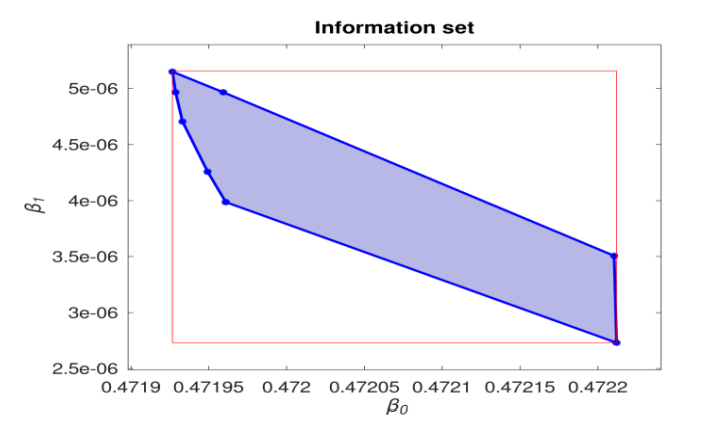
\includegraphics[scale=0.8]{../image/problem8.png}
			\end{tabular}
		\end{center}
		\caption{Информационное множество по модели (10) и (11), интервальная оболочка — красный брус} 
	\end{figure}

	Проведём вычисление параметров линейной регрессии по данным
	интервальной выборки $\textbf{X}_1$ с использованием программ С.И.Жилина
	[8].
	
	Синтаксис вызова программ:
	
	Решение задачи линейного программирования
	$$SS = ir\_problem(A, x, max(w0)*epsilon, lb);$$
	Вершины информационного множества задачи
	построения интервальной регрессии
	$$vertices = ir\_beta2poly(SS);$$
	Внешние интервальные оценки параметров
	модели $y = \beta_1 + \beta_2 * x$
	$$b_{int} = ir\_outer(SS).$$
	
	Входами программы служат значения $mid\:\textbf{X}_1$ и величин неопределённости $\epsilon$, умноженные на расчётное уширение по модели (10) и (11), матрица $A$, составленная из нулевой и первой степеней номеров
	замеров, параметры условной оптимизации. Структура SS содержит
	значения параметров регресии.
	
	\textbf{Коридор совместных зависимостей.} Информационное множество задачи определяется в пространстве параметров. Каждая его точка задаёт зависимость в пространстве переменных. Множество всех таких моделей именуется коридором совместных зависимостей.
	
	Выше мы нашли внешние интервальные оценки параметров модели
	$$mid\:\beta_0 = [4.7193e - 01, 4.7221e - 01],\eqno (21)$$
	$$mid\:\beta_1 = [2.7304e - 06, 5.1571e - 06].\eqno (22)$$
	Подставляя значения (21) и (22) в уравнение регресии, получаем
	$$x(k) = mid\:\beta_0 + mid\:\beta_1 * k, \eqno (23)$$
	где $k$ — номер измерения.
	
	На Рис. 9 приведён коридор совместных зависимостей для модели (23). Визуально видно, что внутри коридор совместных зависимостей можно провести множество прямых.
	
	\textbf{Построение прогноза внутри и вне области данных.} Одним из способов использования регрессионной модели является предсказание значений выходной переменной для заданных значений входной. С помощью построенной выше модели (23) можно получить прогнозные значения выходной переменной в точках эксперимента.
	
	\begin{figure}[H]
		\begin{center}
			\begin{tabular}{ccc}
				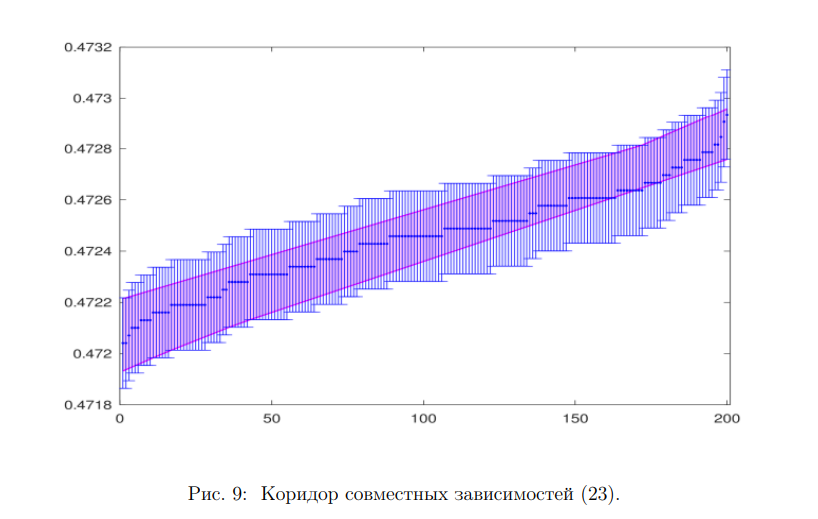
\includegraphics[scale=0.8]{../image/problem9.png}
			\end{tabular}
		\end{center}
		\caption{Коридор совместных зависимостей (23)} 
	\end{figure}
	
	Ценность модели также заключается в возможности её употребления для предсказания выходной переменной в точках, где измерения не производились.
	
	Расширив область определения аргумента для модели (23), можно
	получить оценки для значений выходной переменной (экстраполяция).
	На Рис. 10 сплошной заливкой дан прогноз в том числе за пределами
	данных интервальной выборки $\textbf{X}_1$.
	
	\begin{figure}[H]
		\begin{center}
			\begin{tabular}{ccc}
				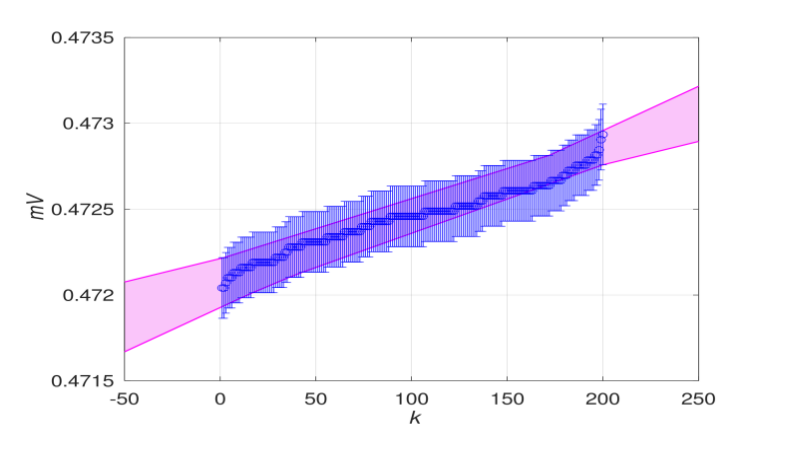
\includegraphics[scale=0.8]{../image/problem10.png}
			\end{tabular}
		\end{center}
		\caption{Коридор совместных зависимостей (23). Построение прогноза} 
	\end{figure}
	
	Следует обратить внимание, что величина неопределённости прогнозов растёт по мере удаления от области, в которой производились исходные измерения. Это обусловлено видом коридора зависимостей, расширяющимся за пределами области измерений, и согласуется со
	здравым смыслом.
	
	\textbf{Уточнение структуры модели. Кусочно-линейная регрессионная зависимость.} Рис. 5 и Рис. 6 регресионных остатков свидетельствуют о том, что линейные регрессионные модели не вполне точно отражают характер зависимости для интервальной выборки $\textbf{X}_1$.
	Наиболее простым способом учёта этого факта является использование кусочно-линейная регрессионной зависимости.
	
	В разделе «Варьирование неопределённости измерений» были вычислены векторы весов $\omega$ расширения неопределённости измерений для достижения совместности — см. Рис. 4. Резкое возрастание весов $\omega$ на границах области определения свидетельствует о несоответствии данных и модели. Эти точки и можно взять как «угловые» для определения линейных участков.
	
	\begin{figure}[H]
		\begin{center}
			\begin{tabular}{ccc}
				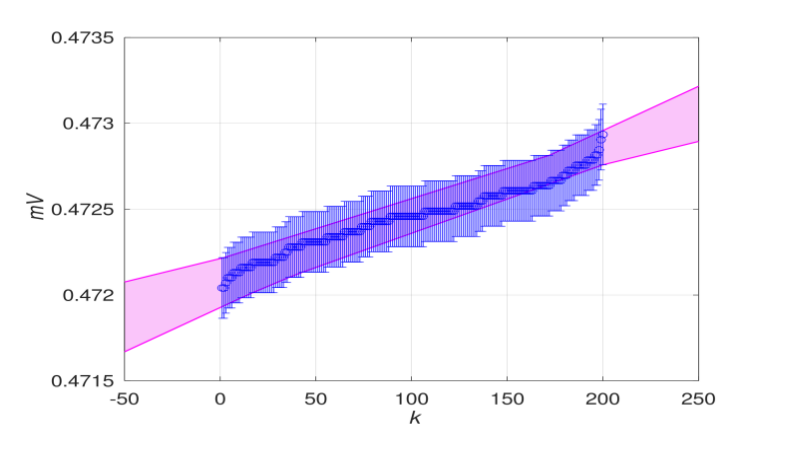
\includegraphics[scale=0.8]{../image/problem10.png}
			\end{tabular}
		\end{center}
		\caption{ Кусочно-линейная регрессионная зависимость} 
	\end{figure}
	
	На Рис. 11 показан пример построения кусочно-линейная регрессионной зависимости и коридора соввместных зависимостей. После вычитания модели, можно переходить к анализу отстатков регресии и другим приёмам анализа.
	
	В более общей постановке ставится задача автоматического определения точек излома [29], [30]. Имеется программное обеспечение
	С.И.Жилина, реализующее идеи этого подхода..
	\section{Реализация}
	\subsection{Описание}
	Данная лабораторная работа была выполнена с использованием языка
	программирования Python 3.10 в среде разработки PyCharm с
	использованием следующих библиотек:
	\begin{itemize}
		\item math - использование математических функций
		\item matplotlib версии 3.7.1 - построение графиков
		\item numpy версии 1.24.2 - использование многомерных массивов
		\item prettytable версии 3.6.0 - вывод таблиц в консоли 
		\item scipy версии 1.10.1 - статические распределения и функции
		\item seaborn версии 0.12.2 - посроение графиков, визуализация
		\item statsmodels - дополнение к scipy, использование статистических вычислений, включая описательную статистику, оценку и вывод статистических моделей
	\end{itemize}
	Отчёт подготовлен с помощью языка LaTEX в редакторе TexStudio.
		\subsection{Ссылка на репозиторий}
		\url{https://github.com/IMZolin/Math-statistics-labs} \ - GitHub репозиторий
	
	\section{Результаты}
	\subsection{Данные выборки}
	Данные для выборки взяты из файла $Channel\_ 1\_400nm\_2mm.csv, \ \varepsilon = 10^{-4}$
	
		\begin{figure}[H]
			\begin{center}
			\begin{tabular}{ccc}
				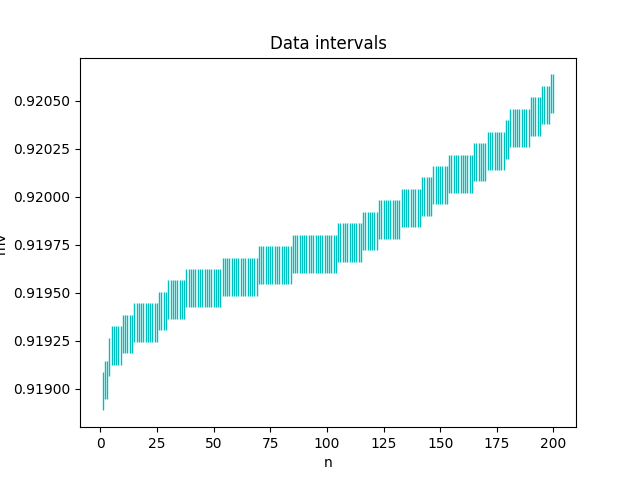
\includegraphics[scale=0.8]{../image/data_and_intervals1.png}
			\end{tabular}
		\end{center}
			\caption{ Диаграмма рассеяния выборки $X_1$ с уравновешенным интервалом погрешности} 
		\end{figure}
	 \subsection{Варьирование неопределённости измерений}
	\begin{figure}[H]
		\begin{center}
			\begin{tabular}{ccc}
				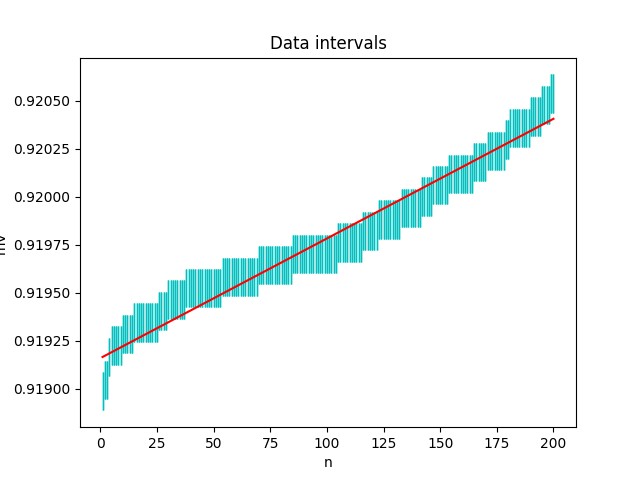
\includegraphics[scale=0.7]{../image/data_and_intervals2.png}
			\end{tabular}
		\end{center}
		\caption{Диаграмма рассеяния выборки $X_1$ и регрессионная прямая по модели (4) и (5)} 
	\end{figure}
	\begin{equation*}
		\sum\limits_{i=1}^n \omega_i = 200,\ \beta_0 = 0.91916, \beta_1 = 6.2333 \cdot 10^{-6}
	\end{equation*}

	\subsection{Варьирование неопределённости измерений с расширением и сужением интервалов}
	\begin{figure}[H]
		\begin{center}
			\begin{tabular}{ccc}
				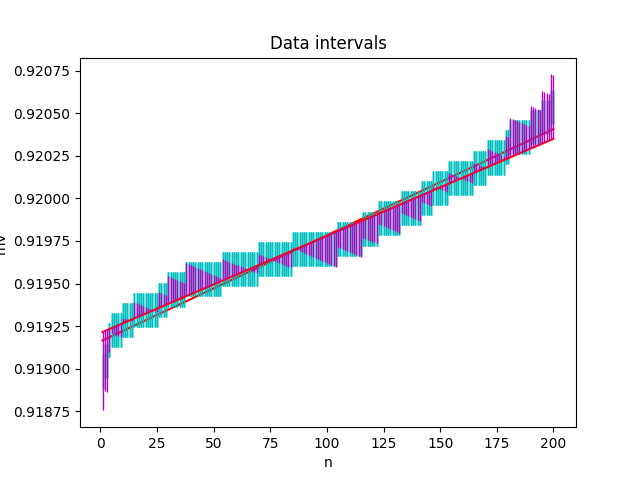
\includegraphics[scale=0.7]{../image/data_and_intervals3.png}
			\end{tabular}
		\end{center}
		\caption{Диаграмма рассеяния выборки $X_1$ и регрессионная прямая по модели (10) и (11)} 
	\end{figure}

	\begin{equation*}
		\sum\limits_{i=1}^n \omega_i = 98.559 ,\ \beta_0 = 0.91921, \beta_1 = 5.6971 \cdot 10^{-6}
	\end{equation*}

	\begin{figure}[H]
		\begin{center}
			\begin{tabular}{ccc}
				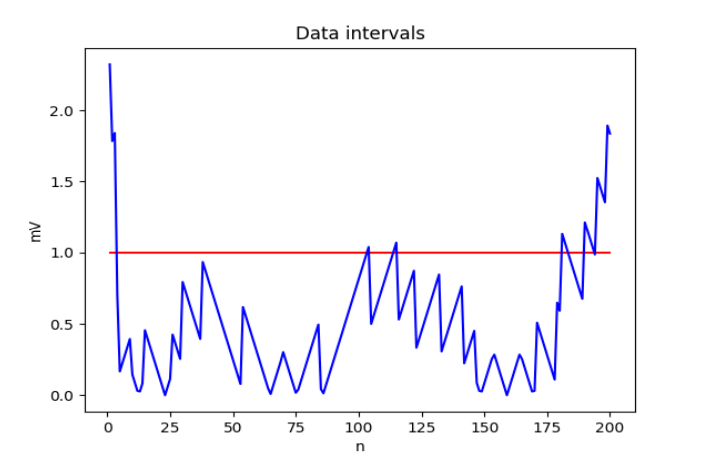
\includegraphics[scale=0.7]{../image/data4.png}
			\end{tabular}
		\end{center}
		\caption{Векторы $\omega_0$ и $\omega_1$} 
	\end{figure}
	
	\subsection{Анализ регресионных остатков}
	\begin{figure}[H]
		\begin{center}
			\begin{tabular}{ccc}
				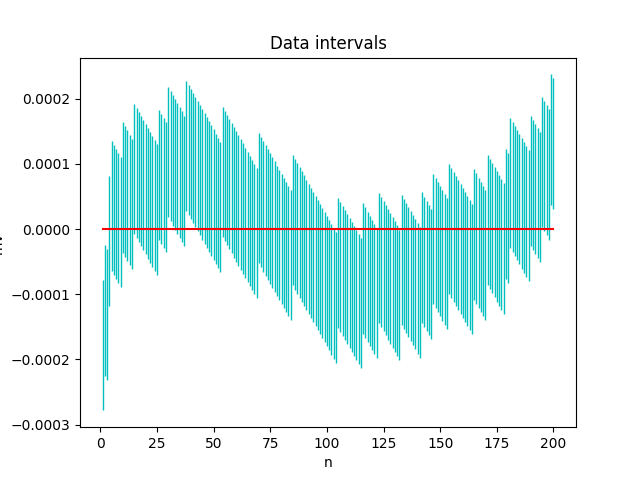
\includegraphics[scale=0.8]{../image/regression_1.png}
			\end{tabular}
		\end{center}
		\caption{ Диаграмма рассеяния по модели (4) и (5)} 
	\end{figure}

	\begin{figure}[H]
		\begin{center}
			\begin{tabular}{ccc}
				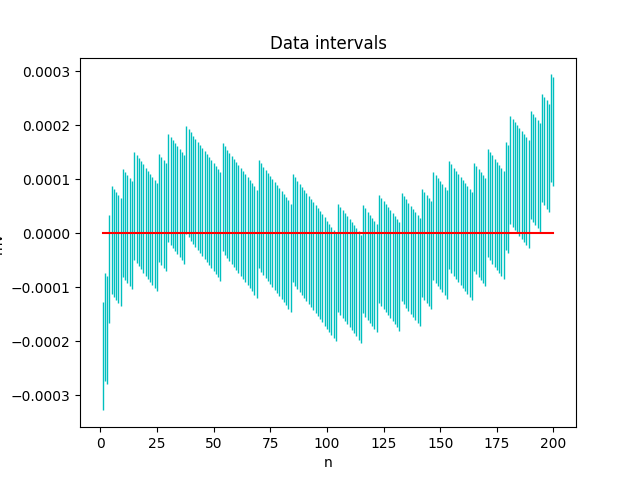
\includegraphics[scale=0.8]{../image/regression_2.png}
			\end{tabular}
		\end{center}
		\caption{Диаграмма рассеяния регрессионных остатков выборки $X_1$ по (10) и (11)} 
	\end{figure}
	\begin{figure}[H]
		\begin{center}
			\begin{tabular}{ccc}
				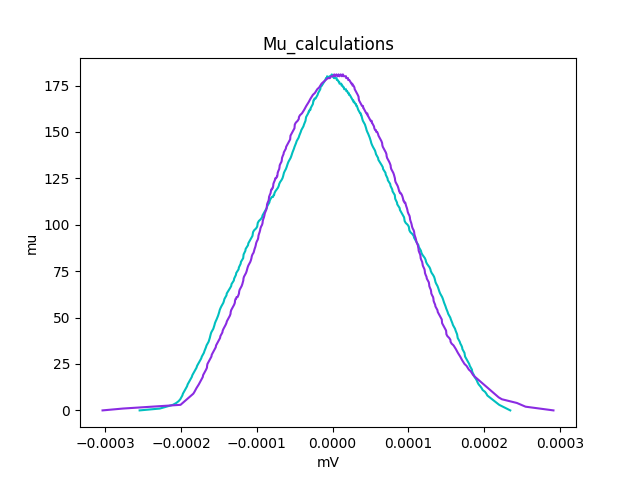
\includegraphics[scale=0.8]{../image/input_mu.png}
			\end{tabular}
		\end{center}
		\caption{Частоты элементарных подинтервалов регрессионных остатков выборки $X_1$ по модели (4) и (5) — синий график, и (10) и (11) — фиолетовый график.} 
	\end{figure}

	Меры совместности регрессионных остатков:
	$mode X_0 = [-0.000007, 0.000007] J_i(X_0) = 0.5335$
	
	$mode X_1 = [-0.000008, 0.000008] J_i(X_1) = 0.6808$
	
	Здесь $X_0, X_1$ – регрессионные остатки выборки $X_1$, вычисленные с использованием разных
	условий оптимизации.
		
	\subsection{Информационное множество задачи}
	\begin{figure}[H]
		\begin{center}
			\begin{tabular}{ccc}
				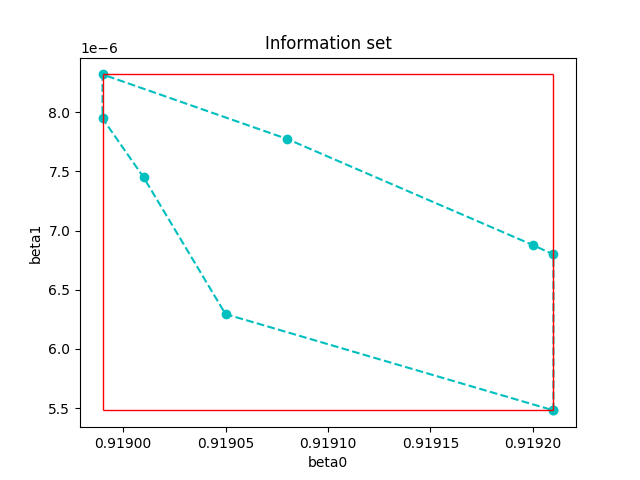
\includegraphics[scale=0.8]{../image/inform_set.png}
			\end{tabular}
		\end{center}
		\caption{Информационное множество по модели (10) и (11), интервальная оболочка — красный брус} 
	\end{figure}
	
	\subsection{Коридор совместных зависимостей}
	\begin{equation*}
		\begin{gathered}
			\midd \boldsymbol{\beta}_0 = [0.91899, 0.91921]\\
			\midd \boldsymbol{\beta}_1 = [5.4802 \cdot 10^{-6}, 8.3358 \cdot 10^{-6}]
		\end{gathered}
	\end{equation*}
	
	Подставляя значения (21) и (22) в уравнение регресии, получаем
	
	\begin{equation*}
		\begin{gathered}
			\midd x(k) = mid \beta_0 + mid \beta_1 \cdot k
		\end{gathered}
	\end{equation*}

	где k — номер измерения.
	
	\subsection{Построение прогноза внутри и вне области данных}
	\begin{figure}[H]
		\begin{center}
			\begin{tabular}{ccc}
				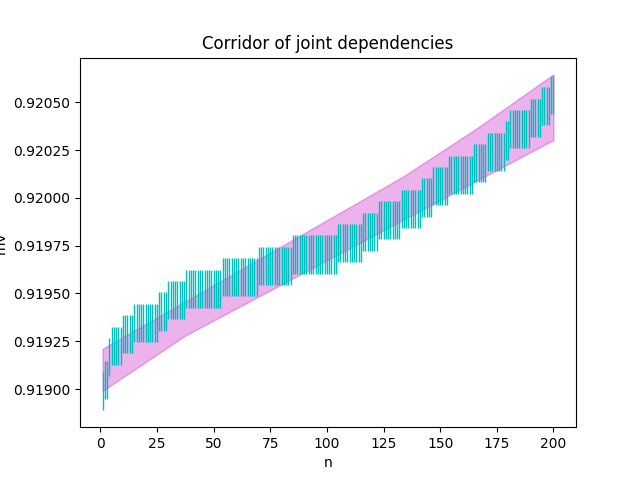
\includegraphics[scale=0.8]{../image/intervals1.png}
			\end{tabular}
		\end{center}
		\caption{Коридор совместных зависимостей (23)} 
	\end{figure}

	\begin{figure}[H]
		\begin{center}
			\begin{tabular}{ccc}
				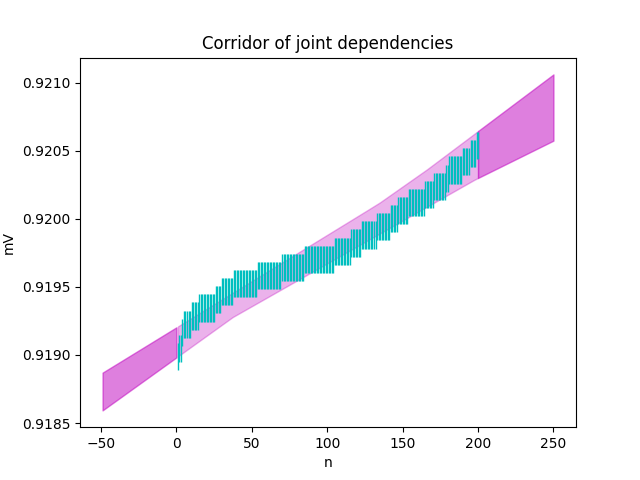
\includegraphics[scale=0.8]{../image/intervals2.png}
			\end{tabular}
		\end{center}
		\caption{Коридор совместных зависимостей (23). Построение прогноза} 
	\end{figure}

	\section{Обсуждение}
	\subsection{Варьирование неопределённости измерений}
	Все компоненты вектора $\omega$ оказались равны 1, то есть, расширения интервалов измерений не понадобилось. Таким образом, величина (4) равна числу элементов выборки. Недостатком полученного решения с единичными значениями $\omega_i$ является неучёт расстояний точек
	регрессионной зависимости до данных интервальной выборки. Таким образом, прямая с параметрами (7) и (8) «не чувствует» отклонений измерений от прямой на концах выборки — неопределённости измерений достаточно велики, чтобы покрыть этот эффект.
	
	\subsection{Варьирование неопределённости измерений с расширением и сужением интервалов}
	Величина меры (4) уменьшилась более, чем в 2 раза. Таким образом, постановка задачи с возможностью одновременного увеличения и уменьшения радиусов неопределённости измерений позволяет более гибко подходить к задаче оптимизации.
	
	\subsection{Анализ регрессионных остатков}
	По результатам вычислений для регрессионных остатков можно сделать вывод, что мода регрессионных остатков по модели с $\omega_i \geq 0$ представляет собой более широкую окрестность нуля. Это означает, что регрессия по этой модели качественнее, нежели по модели $\omega_i \geq 1$.
	
	\subsection{Информационное множество задачи}
	Внешняя интервальная оценка параметра определяется минимальным и максимальным значениями, которых может достигать значение параметра в информационном множестве.
	В совокупности интервальные оценки параметров задают брус, описанный вокруг информационного множества и именуемый внешней интервальной оболочкой информационного
	множества.
	
	\subsection{Коридор совместных зависимостей}
	На Рис. 20 приведён коридор совместных зависимостей для модели (2.54). Визуально видно, что внутри коридор совместных зависимостей можно провести множество прямых.
	
	\subsection{Построение прогноза внутри и вне области данных}
	Следует обратить внимание, что величина неопределённости прогнозов растёт по мере удаления от области, в которой производились исходные измерения. Это обусловлено видом коридора зависимостей, расширяющимся за пределами области измерений, и согласуется со здравым смыслом.
	
	\newpage
	\addcontentsline{toc}{section}{Литература}
	
	\begin{thebibliography}{4}
		\bibitem{s:hist}
		Histogram. URL: \url{https://en.wikipedia.org/wiki/Histogram}
		\bibitem{b:probSectMath}
		Вероятностные разделы математики. Учебник для бакалавров технических направлений.//Под ред. Максимова Ю.Д. --- Спб.: «Иван Федоров», 2001. --- 592 c., илл.
		\bibitem{s:boxplot}
		Box plot. URL: \url{https://en.wikipedia.org/wiki/Box_plot}
		\bibitem{a:nonParamRegr}
		Анатольев, Станислав (2009) «Непараметрическая регрессия», Квантиль, №7, стр. 37-52.
		\bibitem{a:nonParamRegr} М.З.Шварц. Данные технологических испытаний оборудования для калибровки фотоприемников солнечного излучения. 2022.
	\end{thebibliography}

\end{document}